\chapter{Einleitung}

Über die genaue Formatierung der Hervorhebungen sollten wir uns noch
unterhalten. Das ganze kann dann auch so implementiert werden, dass die
Hervorhebungen nur auf den Folien vorhanden sind, \bzw für das Skript nochmal
extra eingestellt werden können. Man könnte hier auch noch zwischen farbig und
nicht farbig unterscheiden. Ich weiß jedoch nicht, ob das sinnv

\section{UsePDFLatex}

Die Vorlage kann nur mit pdflatex übersetzt werden. Es müssen alle Bilder als bitmap zur Verfügung stehen. Um diese bitmaps zu erstellen, kann beispielsweise die in dieser Dokumentation gewählte Vorgehensweise gewählt werden.
\begin{itemize}
	\item Alle Einstellungen des Dokumentes werden in doc\_settings.tex
	gesetzt. So können für Dokument und Bilder die gleichen Einstellungen
	(beispielsweise Schriften) genutzt werden.
	\item Anlegen der Datei figure\_main.tex im Unterordner figs
\end{itemize}


\begin{figure}
	\centering
	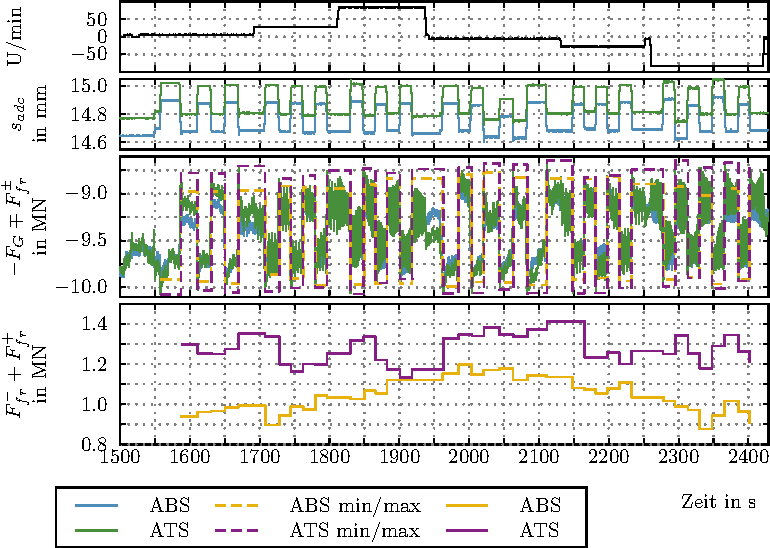
\includegraphics{fig_ExpVariationADC_WeightNFriction}
	\label{fig:WeightNFriction}
	\caption{Gewichtskraft und Reibkraft.}
\end{figure}


\section{Ausgangssituation und Aufgabenstellung}
Im Rahmen der Forschungskooperation zwischen der AG der Dillinger Hüttenwerke und dem Institut für Automatisierung- und Regelungstechnik (ACIN) der Technischen Universität Wien sollen Strategien zur Optimierung des Aufbaus und der Regelung der Richtspaltgeometrie von Warmrichtmaschinen entwickelt werden. Als konkretes Anwendungsbeispiel und  Ausgangspunkt der Untersuchungen dient dazu die Warmrichtmaschine P2 am Standort GTS in Dünkirchen.

%Das Richten von Walztafeln in einer Warmrichtmaschine soll abwickelbare und nicht-abwickel"=bare Ebenheitsdefekte zufolge von Resteigenspannungen reduzieren. Die Walztafel wird dazu wechselseitig über versetzt angeordnete Richtrollen gebogen und dabei gezielt plastifiziert. %Mit einem Richtprozessmodell wird die optimale Anstellung der Richtrollen berechnet und mittels einer elektromechanischen Voranstellung und positionsgeregelter Anstellzylinder eingestellt (vgl. Abb. \ref{fig:schema_aktor} links). Da die Richtmaschine unter der Wirkung der Richtkräfte auffedert, muss die berechnete Zustellung um die Auffederung korrigiert werden. Dabei ist neben der vertikalen Auf"|federung der Anstellschrauben die Querauf"|federung, d.\,h. die Durchbiegung der Richtrollen und die Auf"|federung des Druckrahmens, von Bedeutung.
%Die Richtmaschine federt unter der Wirkung der Richtkräfte auf. Um den gewünschten Richtspalt einzustellen, muss die mit einem Richtmodell berechnete Zustellung um die vertikale Auf"|federung der Anstellschrauben und insbesondere die Querauf"|federung, d.\,h. die Durchbiegung der Richtrollen und die Auf"|federung des Druckrahmens, korrigiert werden.


\begin{bemerkung}
	Eine Bemerkung
\end{bemerkung}

\begin{hinweis}
	Ein Hinweis
\end{hinweis}
Eine wichtige Formel
\begin{markeqn}
\begin{align}
1=1 \ .
\end{align}
\end{markeqn}

Hier folgen einige Literaturreferenzen, z.B. \cite{Henrich1993}
oder\cite{Witte1970}.
